%\documentclass[12pt,preprint]{aastex6}
\documentclass[12pt]{article}

\bibliographystyle{aasjournal}

\usepackage{aas_macros} % need this because not using aastex or emulateapj
\usepackage{graphicx}
\usepackage[suffix=]{epstopdf}
\usepackage{natbib}
\usepackage{amsmath}
%\usepackage{url}
\usepackage{xspace}
\usepackage{fullpage}

%    Make Scientific Notation
\providecommand{\e}[1]{\ensuremath{\times 10^{#1}}}

% make the word Kepler italicized
\newcommand{\Kepler}{\textsl{Kepler}\xspace}

\begin{document}
%%%%%%%%%%%%%%%%%%%%%%

%Measuring Stellar Rotation with K2

\title{Scientific/Technical/Management}
\date{}

\maketitle


% shrink up the space between the "title" and first section heading
\vspace{-1in}

%%%%%%%%%%%%%%%%%%%
\section{Introduction}

Age is key, and nearly impossible to get for field stars. 
Stellar rotation periods are are the most promising tool for constraining the ages of field stars.

kepler makes this possible, get rotation. with K2, new opportunity to do this for range of stellar ages, possibly more than doubling the sample of stars available. K2 also presents unique challenges in data systematics, and shorter baseline means some periods not available... thus we need to use new tools to measure rotation

we propose to measure rotation periods for all light curves from k2. this will produce a value-added dataset for the K2 mission, and extend the science yield from Kepler.

(fill 1st page w/ intro, incl. bold statements of highest level goals)
\clearpage



%%%%%%%%%%%%%%%%%%%
\section{Scientific Motivation}
in new era of both precision exoplanet studies and large surveys of the Milky Way, our ability to better understand stars and their basic properties is key to these larger projects (star formation history of MWY, ages of planet hosts, environment of young-earth like systems, etc).


%%%%%%%%%
\subsection{Rotation Periods from \Kepler and K2}
rotation periods previously were very scarce, had to do with doppler broadening, very rarely could do with photometry.

now with \Kepler we have seen a true revolution, going from hundreds of stars with measured periods from a wide variety of instruments and approaches, to tens of thousands of stars with homogeneous data and analysis. this opens door to understanding a fundamental property of stars 


%%%%%%%%%
\subsection{Age-Dating Field Stars with Rotation}

\citet{skumanich1972}
\citet{barnes2007}
the promise of gyrochronology is key, has ability to get ages with accuracy that rivals any other method (10\%). with Kepler/K2 is a mass production job, but with K2 new challenges in the data are lurking

\begin{figure}[!th]
\centering
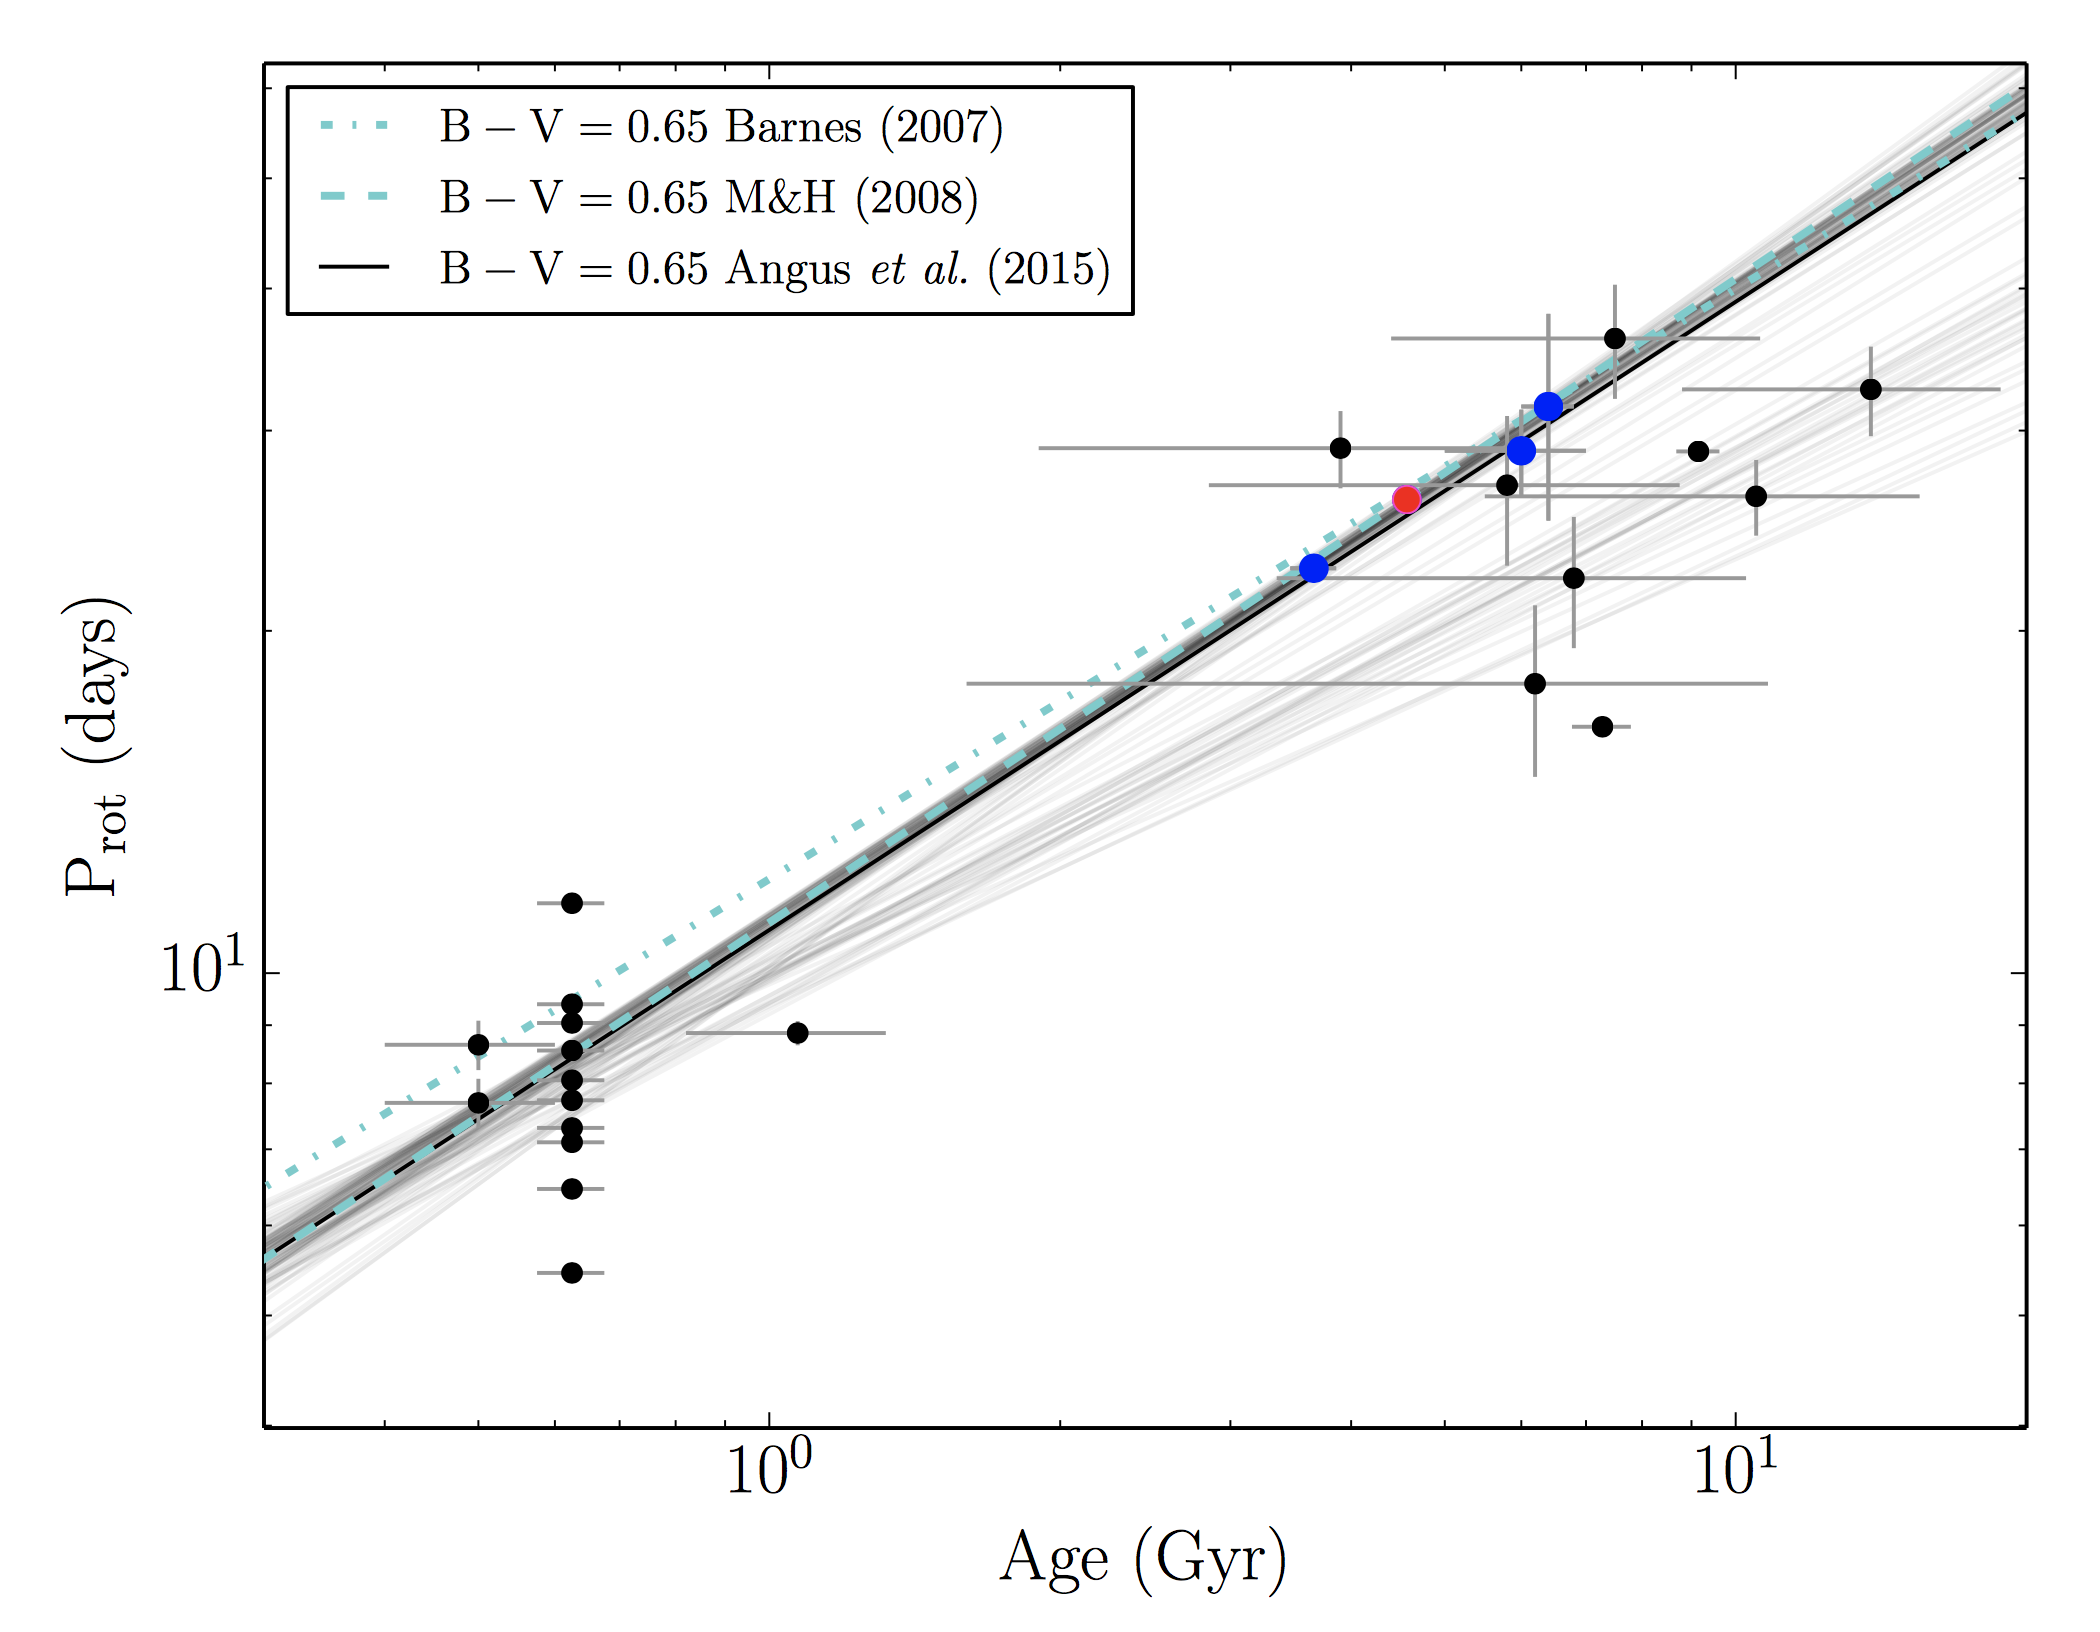
\includegraphics[width=4.5in]{angus2015_fig6.png}
\caption{figure 6 from \citet{angus2015}, showing new gyrochronology relation calibrated using \Kepler asteroseismic targets
}
\label{fig:gyro}
\end{figure}



%%%%%%%%%
\subsection{A Mysterious Period Bimodality}

Then this weird thing appeared, which is an open mystery - a bimodal period distribution - whoa \citep{mcquillan2013}. this was then extended to higher masses by \citet{davenport2017}. Explanations are either a break from single spin-down law (possibly from different initial periods, or some new physics maybe due to chemical abundances) or represents an age bimodality of local stars.

 Since this effect is seen only within 300pc so far (and only within Kepler data) due to sample properties, cannot be sure what spatial or compositional dependence this has, need a sample that spans a wider spatial area and more ages of stars

\begin{figure}[!th]
\centering
\makebox[\textwidth][c]{ % sloppy hack to make figure slightly overflow
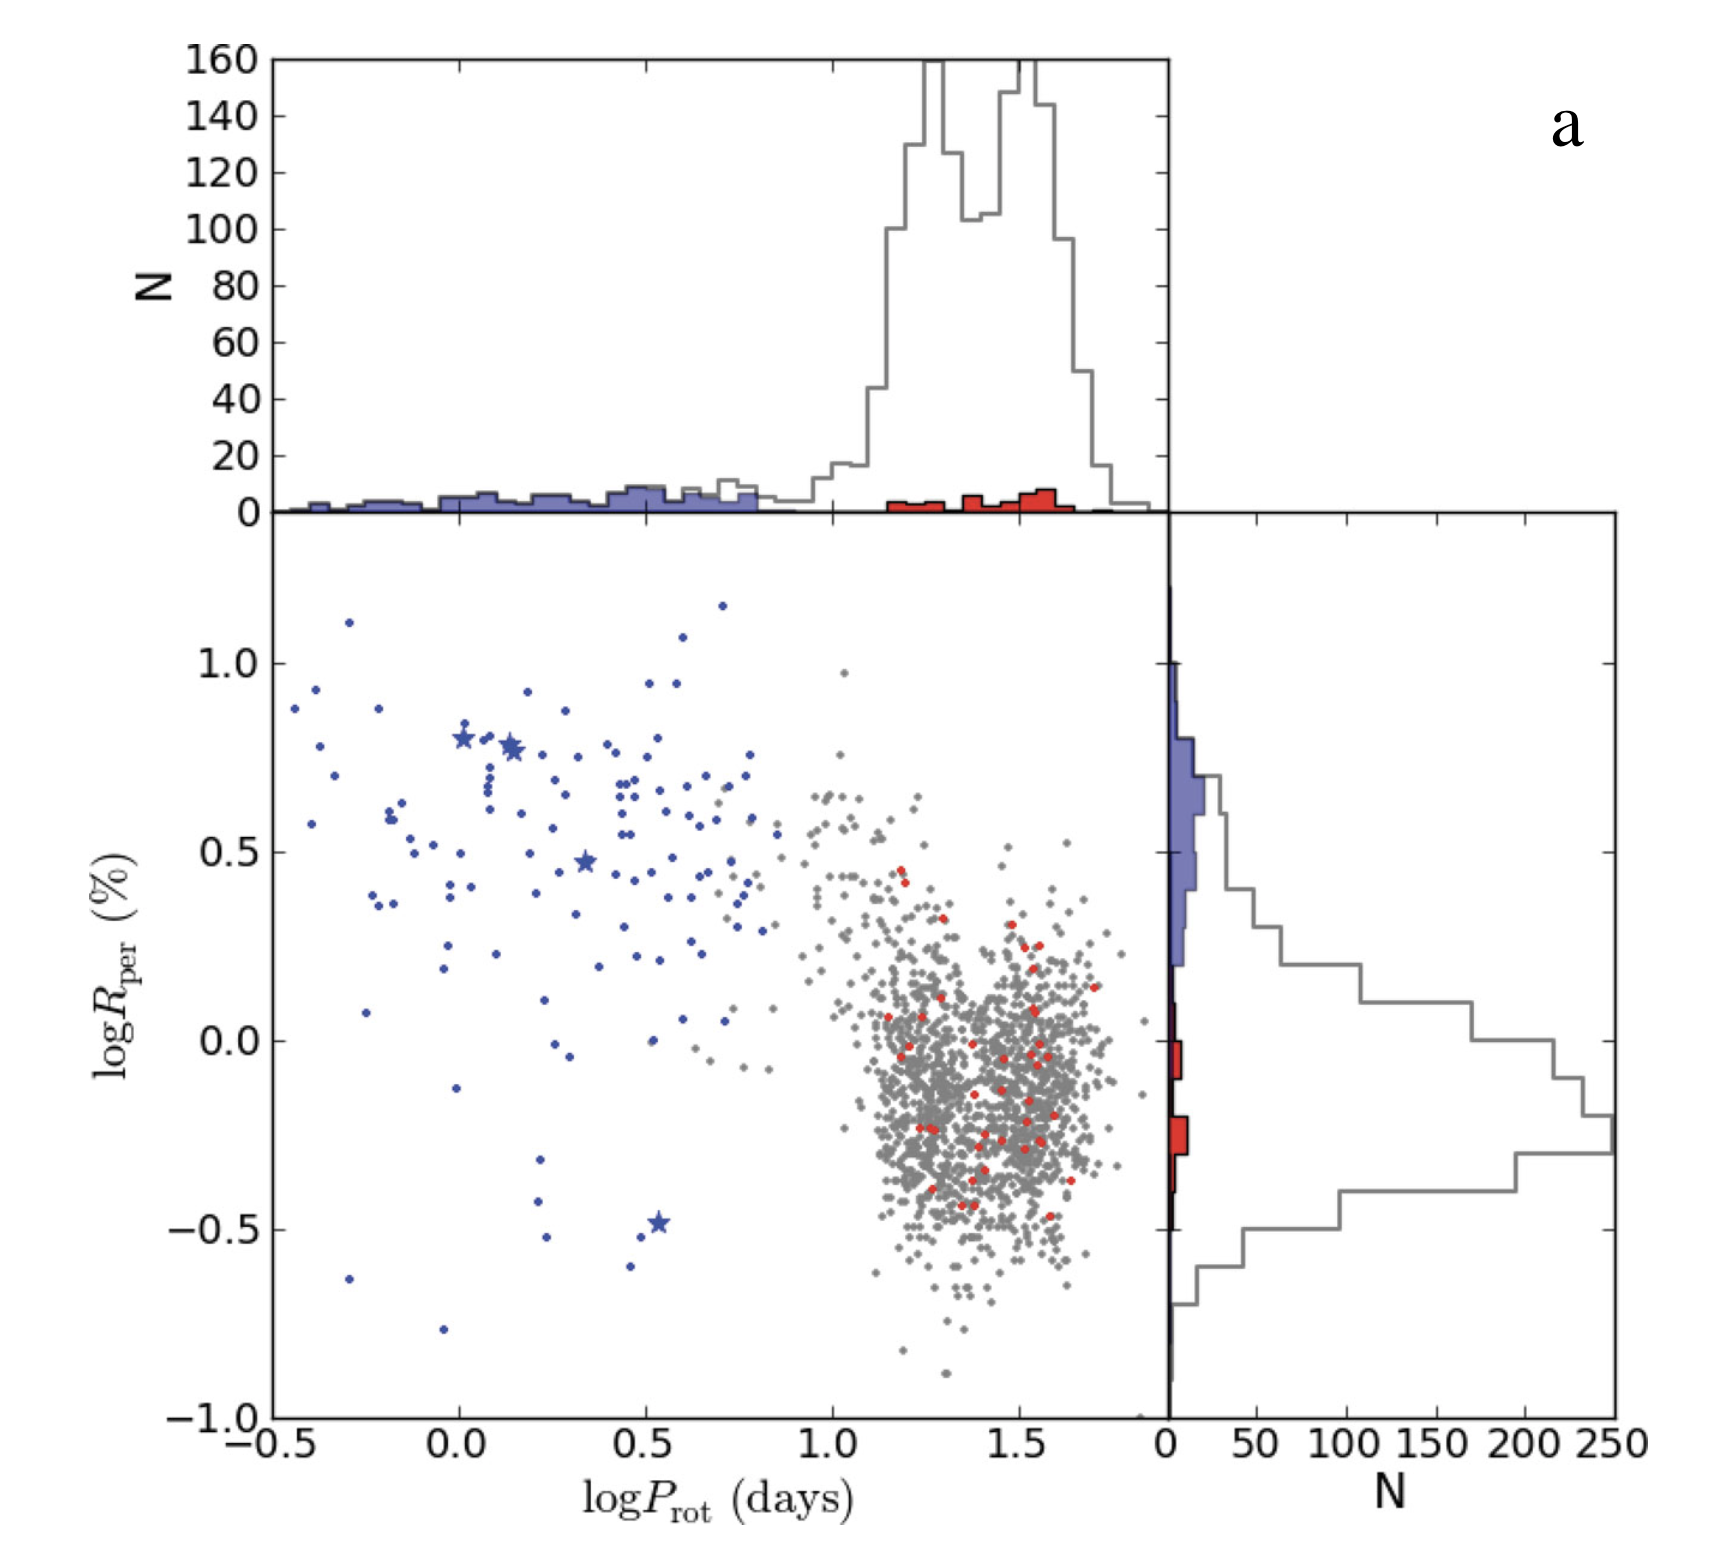
\includegraphics[width=3in]{mcquillan2013_fig9.png}
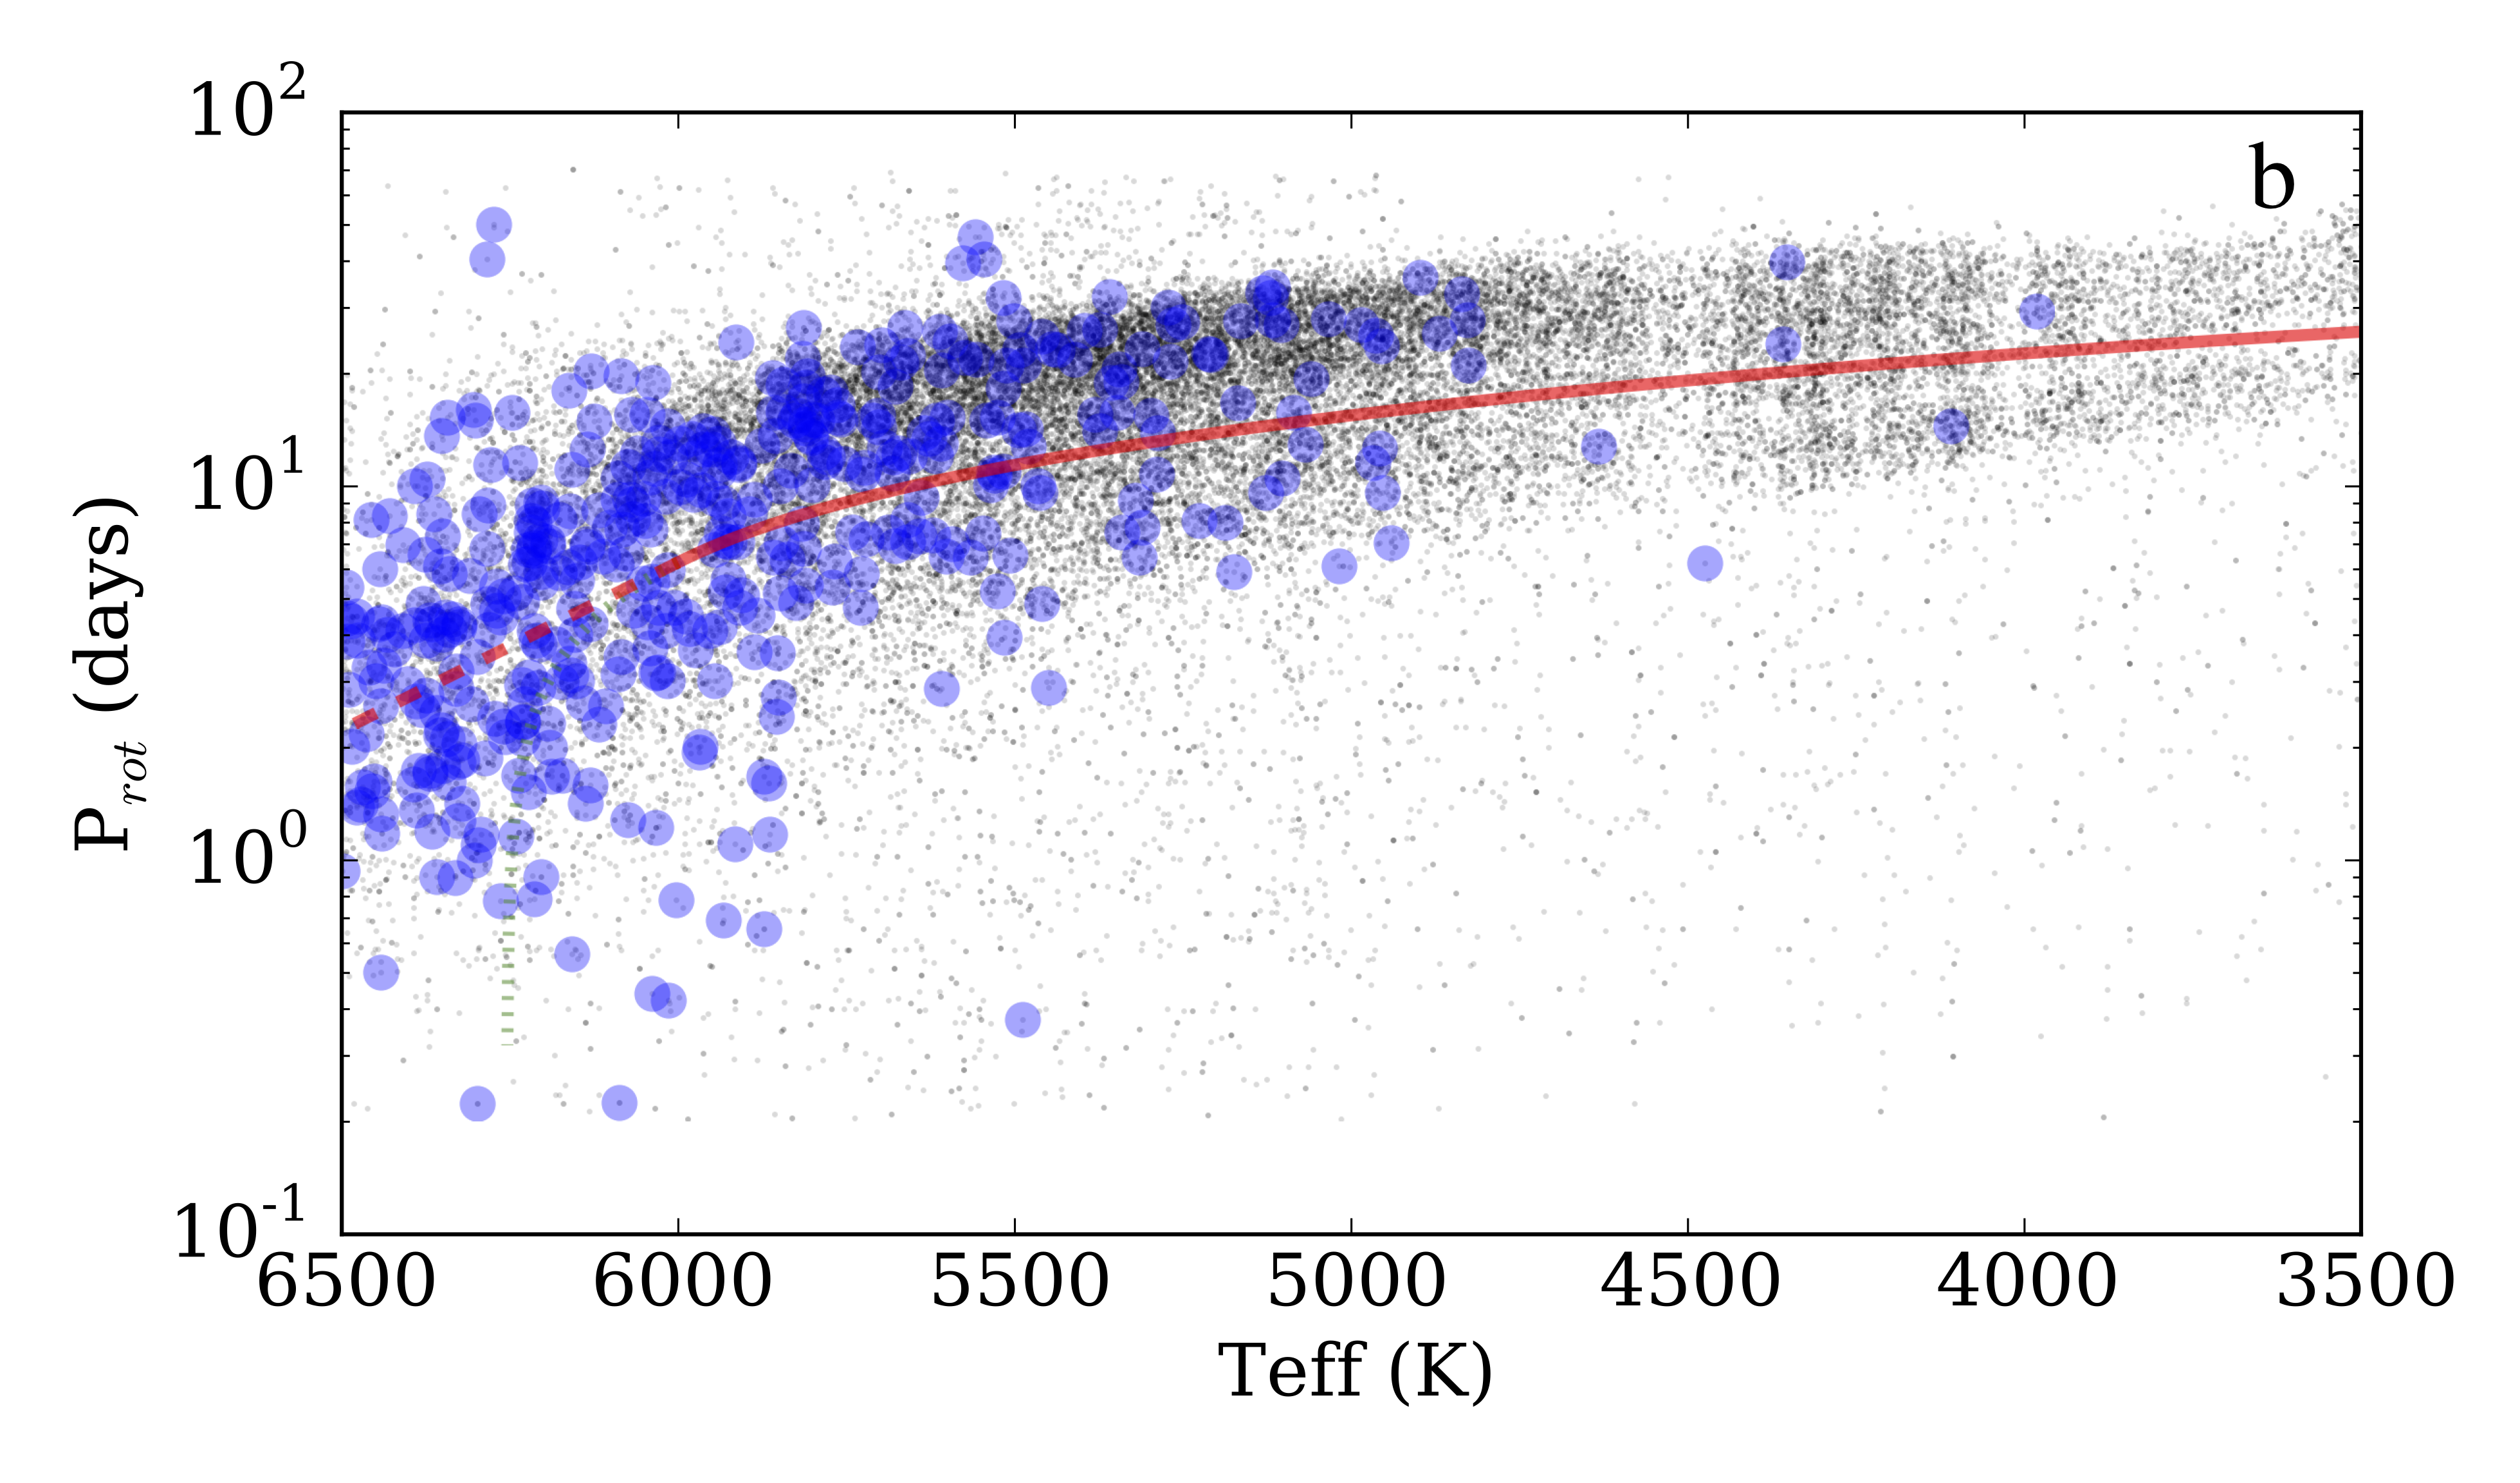
\includegraphics[width=4in]{davenport2016_fig3}
}
\caption{
Left: figure 9 from \citet{mcquillan2013}, showing discovery of bimodality in rotation periods from \Kepler M dwarfs.
Right: figure 3 from \citet{davenport2017}, showing bimodality in rotation periods from \Kepler extends from cool M dwarfs through hotter solar-type stars.
}
\label{fig:bimodal}
\end{figure}



%%%%%%%%%%%%%%%%%%%
\section{Proposed Research} 
%%%%%%%%%
\subsection{Measuring Rotation from K2 Using the Systematics-Insensitive Periodogram }
we propose the first systematic study of stellar rotation periods from the K2 data. 

this will include $\sim$XXXXX stars from Campaigns 0-16. This includes data for multiple stellar clusters that were taken as part of the Guest Observer program.

data will be reduced using SOME FLAVOR of K2 pipeline.


the \citet{angus2016} rotation period pipeline will then be applied to every light curve. we will generate and save every periodogram for potential follow-up analysis of differential rotation and multi-period systems

spurious signals from transits and flares will be filtered out (some smoothing or high-freq removed in the SIP?)

for stars with good period recovery, fourier fits will identify eclipsing binaries and pulsating systems (or something like this)


\begin{figure}[!th]
\centering
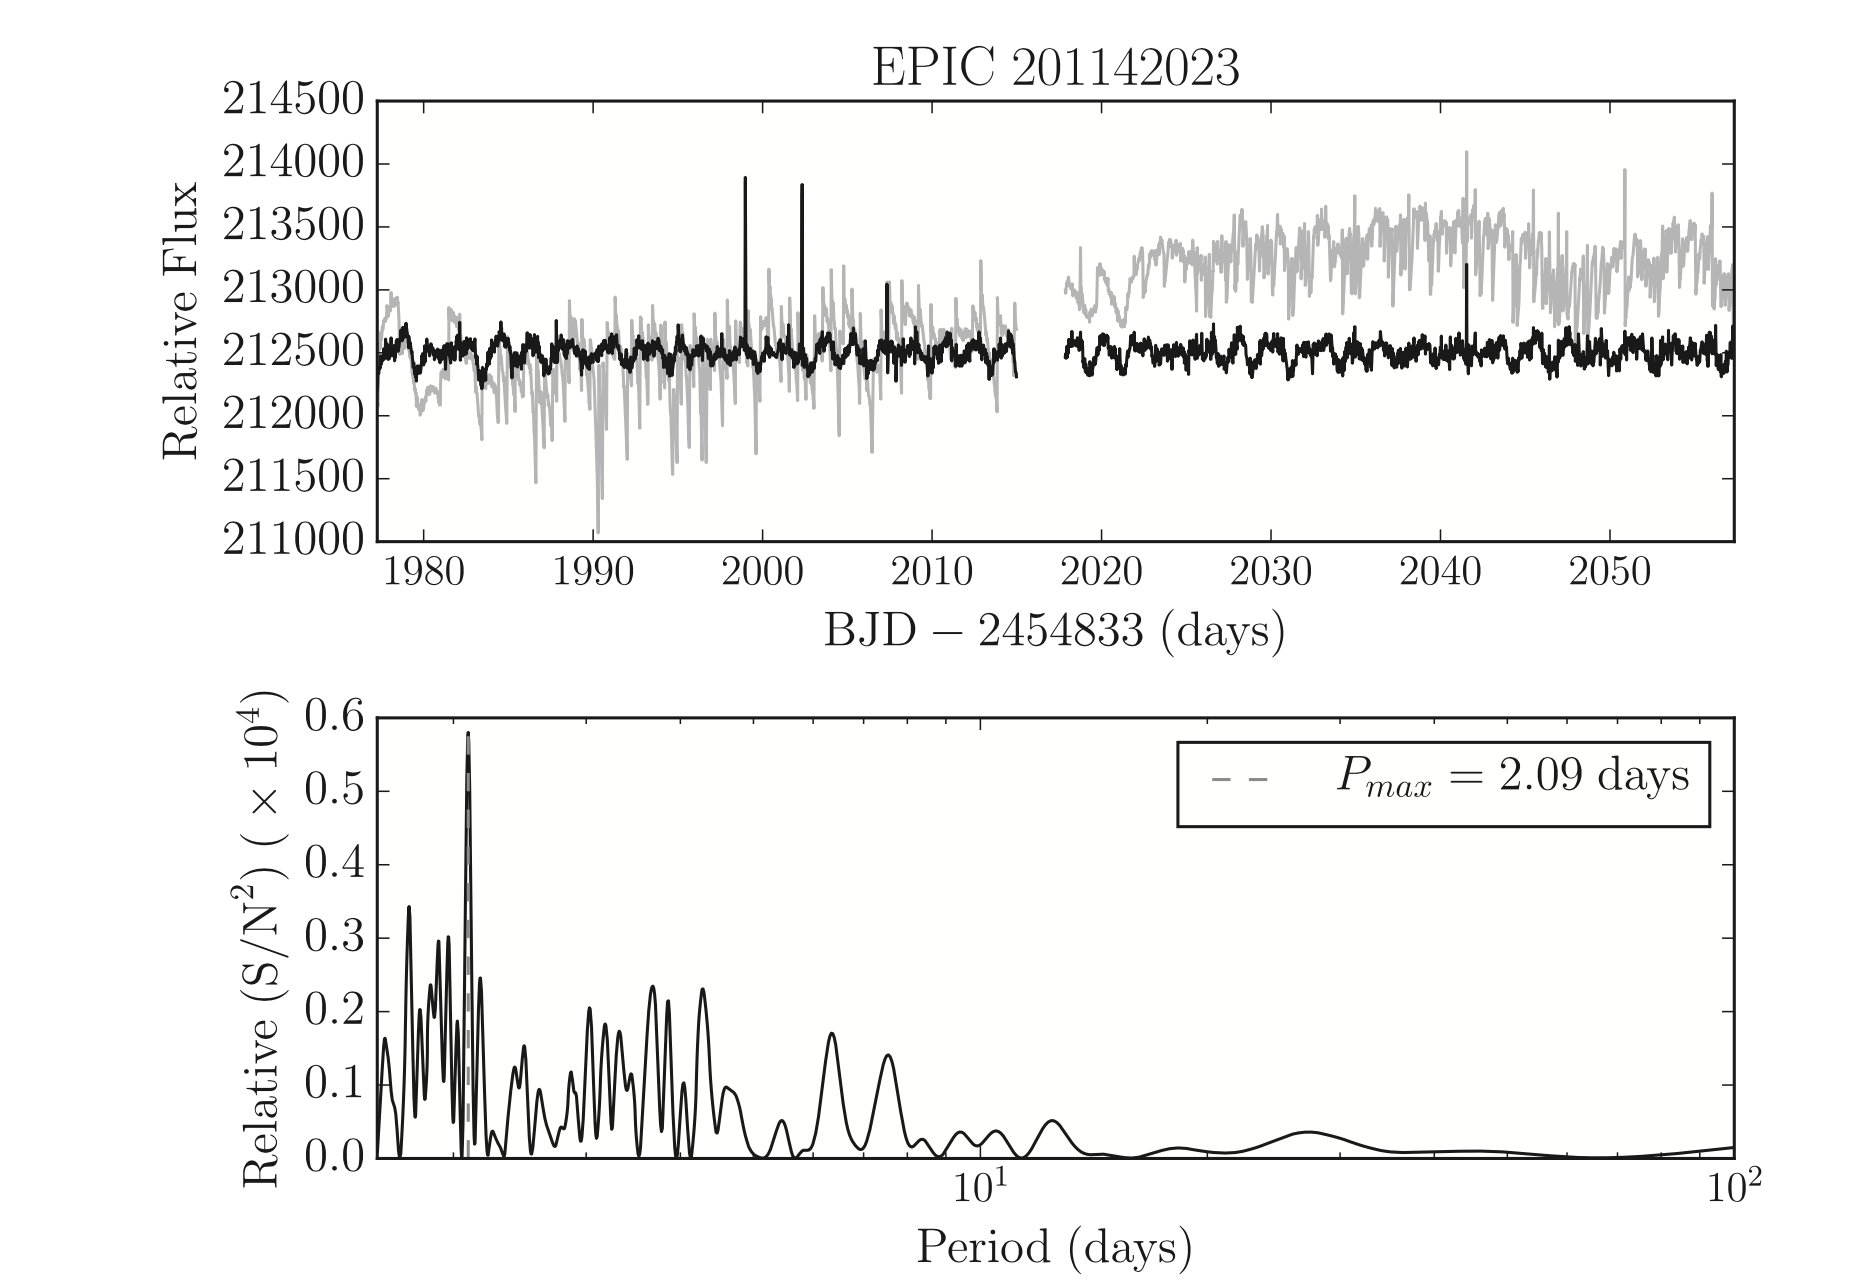
\includegraphics[width=4in]{angus2016_fig6.png}
\caption{
figure 6 from \citet{angus2016}, showing the processing of the light curve and resulting SIPeriodogram. more simple methods give erroneous periods for this object of either 3 days via ACF, or 59 days via normal Lomb-Scargle methods.
}
\label{fig:sip}
\end{figure}




%%%%%%%%%
\subsection{Exploring the Period Bimodality}
by combining our sample with the distances provided in the forthcoming Gaia DR2 catalog, we will be able to extend the methodology of \citet{davenport2017} to filter our subgiants and binary stars for our entire sample.

we then can make 3d exploration of period distribution, to see if the bimodality exists for all field stars near the sun.

the big goal here is to decide which explanation is correct!

\begin{figure}[!th]
\centering
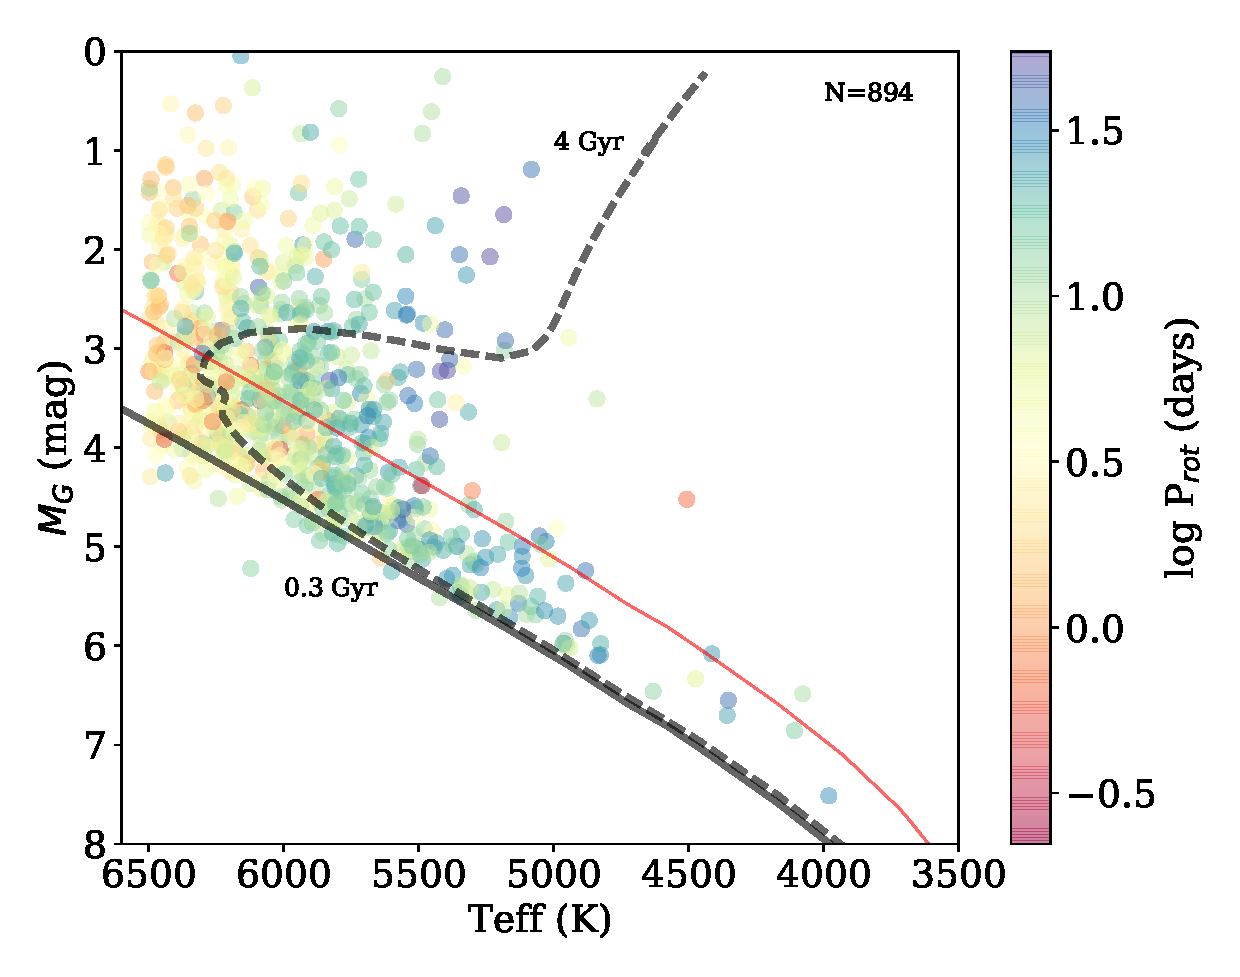
\includegraphics[width=4in]{davenport2016_fig2}
\caption{figure 2 from \citet{davenport2017}, showing temperature from KIC versus absolute magnitude from Gaia}
\label{fig:cmd}
\end{figure}




%%%%%%%%%
\subsection{Mapping Ages in each Field}
our catalog of rotation periods from K2, combined with existing catalogs from Kepler, we will have the largest set of rotation periods ever to use for population analysis. using new technique being developed by Ruth (Chronometer) we will have improved age estimate for every star based on single rotation values. then we combine this to get age distribution within each K2 field.

Demonstration figure?

discussion of improved gyrochronology calibration?

this is partially an extension of the period bimodality work (if it's an age effect), but to create a detailed map of the ages of these field stars at a range of galactic latitudes in the 17 pencil-beams available from K2. combining with the periods from Kepler, will be even better. ultimately we'd like to compare to the age distributions in simulations of these fields from TRILEGAL, and from other age indicators (asteroseismology, flare ages, etc)



%%%%%%%%%%%%%%%%%%%
\section{Team Qualifications}
PI Davenport has used \Kepler to conduct the largest survey to-date of stellar activity from flares, as well as multiple investigations of starspots and their evolution with time using \Kepler data. From these studies, Davenport has developed an age model for flare activity that will be directly comparable to the ages and starspot amplitudes derived from this study. He has also recently discovered the rotation period bimodality first noted with \Kepler M dwarfs by \citet{mcquillan2013} extends to G and K dwarf stars \citep{davenport2017}.
Davenport previously collaborated on NASA ADP grant NNX09AC77G to characterize NIR variability using the 2MASS Calibration Scan Point Source Working Database \citep{davenport2012,davenport2015a}.
He has mentored numerous students on projects using \Kepler data, resulting in student-led publications such as the flare activity of a unique M dwarf binary system GJ 1245AB \citep{lurie2015}, and exploring the poorly understood origins of wide binary stars through stellar rotation (R. Clarke in prep). He will manage the overall project, and lead the investigation and publication of the period bimodality exploration. 

Co-I Angus is an expert in the extraction of periodic signals from \Kepler data using Gaussian Processes \citep{angus2016c} and other cutting-edge statistical techniques. She is the author of tools for generating Systematics-Insensitive Periodograms for both \Kepler and K2 data \citep{angus2016}, as well as new gyrochronology calibrations using \Kepler asteroseismic targets \citep{angus2015}. She will lead the effort to measure and publish rotation periods for all K2 sources, and lead the graduate student in measuring ages for field stars.

other Co-Is?

%%%%%%%%%%%%%%%%%%%
\section{Relevance to NASA Programs}
history of MWY, age of planet systems, TESS



%%%%%%%%%%%%%%%%%%%
\section{Plan of Work}
{\bf Year 1:} process all rotation period data
\\
{\bf Year 2:} write papers 



\clearpage
%\pagestyle{empty}

\bibliography{/Users/davenpj3/Dropbox/references}


\end{document}

